\documentclass[a4paper]{scrartcl}
%\documentclass[a4paper, 10pt]{scrartcl}
\usepackage[czech]{babel}
\usepackage[utf8]{inputenc}
\usepackage{a4wide}

\usepackage{graphicx}
\usepackage{url}


\title{Spánek, zdraví a spánková hygiena}
\subtitle{}
\author{Iveta Terezie Pelikánová}
\date{}

\begin{document}
\maketitle 

Spánek je přirozenou součástí života lidí i zvířat. 
Jde o fyziologický stav vědomí, který je charakteristický útlumově-relaxační
fází organismu, kdy dochází k utlumení některých funkcí (snížení teploty,
snížení krevního tlaku, uvolnění svalstva a další). Dále je charakteristický snížením
pohybu a zavřenýma očima, což nemusí být typické pro některá zvířata. 
Potřeba spánku se během života mění a je nejen závislá na věku, ale také na vnějším
okolí jedince. Obecně se spánkový rytmus vyvíjí s rozvojem centrálního nervového
systému. Novorozenci spí kolem 20ti hodin denně. Od konce prvního roku života se délka
spánku zkracuje na 14 -- 15 hodin a postupně se střídání spánku a bdělosti přetváří do
tzv. bifázického rytmu, kdy dítě spí především v noci a tento spánek je doplněn
maximálně o dva krátké úseky spánku přes den. Předškolní děti spí průměrně 12 hodin. 
S nástupem do školy se utváří monofázický rytmus spánku. Adolescenti spí průměrně 9 
hodin. V dospělosti spí lidé průměrně 7 -- 8 hodin denně. V poslední době dochází 
k mírnému prodlužování spánku mezi 25. a 30. rokem života. S rostoucím věkem často 
dochází ke snížení kvality spánku a často také ke zkracování délky spánku.\cite{Truhlarova_biochemie_spanku,Barosova_fyziologie_spanku}\\

Během 20. století byl spánek intenzivně studován. Pomocí EEG (elektroencefalogram)
byly objeveny dvě stádia spánku, které se v cyklických rytmech během spánku opakují.
Rozlišujeme fázi REM, z anglického \emph{rapid eye movements}, a NREM, z anglického \emph{non-rapid eye movements}.
REM fáze je doprovázena rychlými pohyby očí a větší uvolněností svalů. V této fázi
dochází také ke snění. Frekvenční mozková aktivita se zvyšuje a dostává se do frekvencí $\alpha$ a $\beta$. Oproti svalovému uvolnění se zrychluje dech a zvyšuje tepová frekvence, která se blíží bdělému stavu. \cite{Barosova_fyziologie_spanku,Vitu_ukladani_ke_spanku,brain_basics_ninds}
NREM fáze je charakteristická velkým klidem, nízkým krevním tlakem a 
tepem, někdy se jí také přezdívá hluboké spaní. Hypofýza produkuje velké množství růstového hormonu 
somatotropinu. Tuto fázi dále dělíme do čtyřech kratších fází NREM1 --
NREM4. První fáze NREM1 je přípravou na hluboký spánek, zpomaluje se 
tepová a dechová frekvence a svaly se postupně relaxují. Fáze trvá 
několik málo minut. Ve druhé fázi NREM2 dochází mimo hlubší relaxace 
ke zpomalení mozkové frekvence. Na EEG se zobrazují tzv. spánková 
vřeténka - krátké úseky rytmických vln. NREM3 se označuje jako středně 
hluboký spánek. V této fázi se nám mohou také zdát sny, které si ale 
nepamatujeme. Fáze NREM4 je fází hlubokého spánku. Dochází k úplné 
svalové relaxaci a obnově fyzických sil. Mozková činnost se projevuje
$\delta$ vlnami. Pokud člověka probudíme v této fázi spánku může
trpět dezorientací. 
\cite{Truhlarova_biochemie_spanku,Vitu_ukladani_ke_spanku,brain_basics_ninds,wikipedie_sleep}

Na obrázku \ref{fig:vlny_mozkove} je vidět přehledně mozková aktivita.
Na obrázku \ref{fig:hypnogram_spanku} jsou zobrazeny spánkové cykly -- 
střídání REM a NMREM fází během 8hodinového spánku dospělého člověka.
Jeden spánkový cyklus trvá průměrně 90 -- 120 minut a jejich délka se
během noci zkracuje.
Doba strávená v hlubokém spánku se během noci zkracuje. Na hypnogramu je
také možné pozorovat, ve kterých fázích, se nám zdají sny a proč si
tedy za jednu noc můžeme pamatovat více snů. 

        \begin{figure}
            \centering
            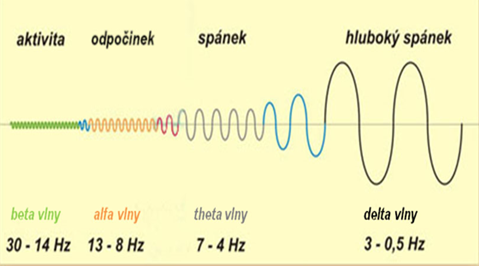
\includegraphics[width=0.8\textwidth]{aktivitamozku.png}
            \caption{Přehled mozkových aktivit.\cite{mozkove_vlny_reference}}
            \label{fig:vlny_mozkove}
        \end{figure}
        
        \begin{figure}
            \centering
            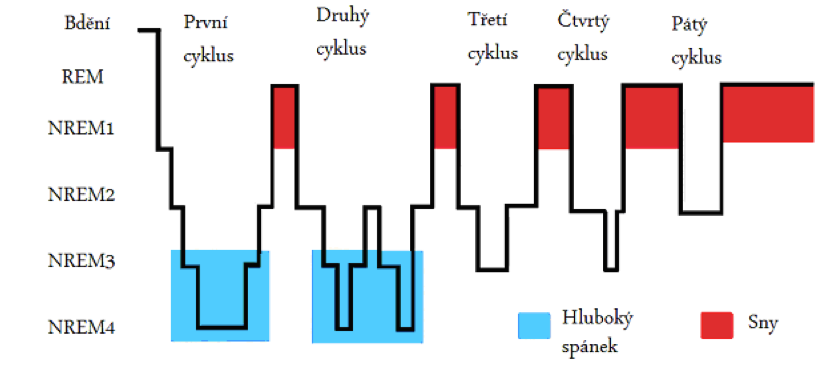
\includegraphics[width=0.9\textwidth]{hypnogram_8hod.png}
            \caption{Hypnogram spánkových cyklů pro 8hodinový spánek.\cite{Vitu_ukladani_ke_spanku}}
            \label{fig:hypnogram_spanku}
        \end{figure}

Teď již víme, kolik průměrně lidé spí a jak vypadají spánkové cykly.
Co ale spánek ovlivňuje a co může způsobit nedostatek spánku či 
nekvalitní spánek? 
Spánek posiluje imunitní systém, protože dochází ke zvýšení
produkce signálních proteinů imunitního systému - cytokinů. \cite{imunitni_system_sleep}
Dále dochází k plasticitě mozku a posilování paměti. 
Spánek pozitivně ovlivňuje
koncentraci, produktivitu a kreativitu. Zlepšuje metabolismus, snižuje
riziko obezity, srdečních chorob, metabolického syndromu, působí
preventivně proti vzniku depresím a duševním onemocněním. \cite{why_we_sleep_fletcher}

V porovnání s pozitivními vlivy spánku jsou v literatuře více
popsány negativa nedostatku spánku a poruchy
spánku. Nedostatek spánku, tzv. spánková deprivace, může být akutní 
či chronická. Akutní spánková deprivace vzniká při dlouhodobém bdění po několik dní. Fyziologicky dochází ke zvýšení hladiny kortizolu v krvi a zvýšení krevního tlaku, klesá výkon jedince a schopnost učit
se. Jedinec začíná být podrážděný, nervozní, a dochází ke snížení
imunity. Chronická spánková deprivace vzniká při dlouhodobém nedostatečném
spánku. Častá je únava jedince během dne, nesoustředěnost, je
prokázáno, že při chronické spánkové deprivaci dochází k omezení 
citového prožívání. Statisticky častěji touto deprivací trpí lidé
s večerním chronotypem, protože jejich přirozená aktivita je dlouho
do noci, ale ráno musí často kvůli pracovním povinnostem vstávat 
dříve než by potřebovali. \cite{Hostalkova_spanek_odpocatost} Na chronickou deprivaci si organismus poměrně dobře zvykne, bohužel to
ale neznamená, že by to jedinci vyhovovalo. Dlouhodobý nedostatek
spánku může vést k nadváze, zvyšuje se riziko diabetu a metabolického syndromu, rozvinutí deprese a úzkostí, 
snižuje se imunita. \cite{nhs_lack_of_sleep}\\

Mimo délky spánku je také důležitá jeho kvalita. Je mnoho parametrů,
které ovlivňují kvalitu spánku. Mezi tyto parametry patří věk a
tělesná konstituce jedince, pracovní vytížení, fyzická aktivita,
životospráva a celkový styl života. Důležitými parametry jsou také
genetické predispozice, teplota, tlak vzduchu, osvětlení, hluk
a matrace. \cite{Barosova_fyziologie_spanku} Důležitým kritériem 
ovlivňující kvalitu spánku v dnešní době je stres. Míra stresu je 
často spojena právě s pracovním vytížením a vysokým očekáváním 
společnosti. \\

Mezi první pomoc při nedostatečného
spánku je důsledné dodržování spánkové hygieny. Spánková hygiena často
může vyřešit problémy ze spánkem bez nutnosti nasazení léků. Zde je
současně třeba opatrnosti, pokud problémy přetrvávají je třeba vyhledat lékaře, který může diagnostikovat rozsáhlejší zdravotní 
problémy a nasadit odpovídající léčbu.\\

\textbf{Zásady spánkové hygieny} \cite{brain_basics_ninds, nhs_lack_of_sleep, nhs_sleep_tips,medical_news_sleep_tips}
    \begin{itemize}
        \item Chodit spát a vstávat v přibližně stejnou dobu každý den
            včetně víkendů
        \item Cvičit 20 -- 30 minut denně, nejpozději několik hodin
            před spaním
        \item Vyvarovat se konzumaci povzbuzujících látek před spaním:
            káva, kofein, nikotin
        \item Nepít alkohol před spaním
        \item Nejíst těžká jídla těsně před spaním
        \item Dodržovat vyvážený zdravý jídelníček
        \item Relaxovat před spaním -- například koupel, čtení,
            relaxace
        \item Teplota ložnice kolem 20$\,^{\circ}$C
        \item Pravidelné větrání ložnice
        \item Spát v tmavé místnosti
        \item Neusínat u televize či rádia, snížit hlučnost prostředí
        \item Umístit počítač do jiné místnosti
        \item V posteli pouze spát a nepolehávat během dne
        \item Vyvarovat se používání telefonů a tabletů v posteli a 
            nejlépe i hodinu před ulehnutím
        \item Vytvořit si spánkový diář
        \item Snížit stres
    \end{itemize}

Dodržovat všechna pravidla spánkové hygieny se může zdát být velmi
náročné. Je dobré o dodržování spánkové hygieny usilovat, ale
je třeba si uvědomit, že cílem je kvalitní spánek a že naše přílišná
snaha o dodržení pravidel může naopak vést ke stresu a problémům 
s usínáním. Každý člověk by si měl najít svoji optimální dobu spánku, někteří jedinci 
prostě potřebují méně či více spánku než jiní pro subjektivní pocit odpočatosti.
Důležitým aspektem je také aktuální zdravotní stav.
A spánková pravidla je vhodné upravit 
dle subjektivních možností a preferencí. Spánek je tím nejjednodušším
lékem, který můžeme každý naordinovat sám sobě a prospat se tak k 
lepšímu zdraví.


\vspace{36pt}
\indent Tento text byl vypracován k udělení zápočtu z 
předmětu \emph{Člověk a zdraví}.


%------ LITERATURA
\newpage
%\bibliographystyle{acm}
\bibliographystyle{unsrt}
\bibliography{reference}
%------ /LITERATURA

\end{document}
